



\begin{table}[ht]\centering
\caption{Metrics Summary\label{tab:metric_summary}}
% \addcontentsline{lot}{table}{Metrics Summary}
\resizebox{.8\textwidth}{!}{%
\begin{tabular}{@{}lp{.35\linewidth}l@{}}
\toprule
Metric Class & Description & Common Measurements \\ \midrule
Structural & Metrics based on the structure of the attack graph; used to identify attributes like shortest path, mean path length, or total number of paths. & SP, NP, MPL \\
Time-Based & Metrics that quantify time expectations for attributes like compromise, recovery, or incident response. & MTTF, MTTB, MTTR \\
Probability-Based & Metrics that associate probabilities attack paths to quantify the security of the network. & NR, PP, EPL \\
Temporal & Metrics that examine  vulnerability age on the system. & TAG \\ \bottomrule
\end{tabular}%
}
\end{table}

% 



NIST 800-55\cite{Swanson_Bartol_Sabato_Hash_Graffo_2003} describes security metrics as "\textit{tools designed to facilitate decision making and improve performance and accountability through collection, analysis, and reporting of relevant performance-related data. IT security metrics must be based on IT security performance goals and objectives.}" This section reviews some of the available security metrics from the literature loosely grouped by each Cybok heading, along with properties that have been used to characterize these metrics. 

\subsection{Existing Security Metrics Taxonomies}\label{sec:background:existing_metrics_taxonomies}



\begin{figure}[ht]
\centering
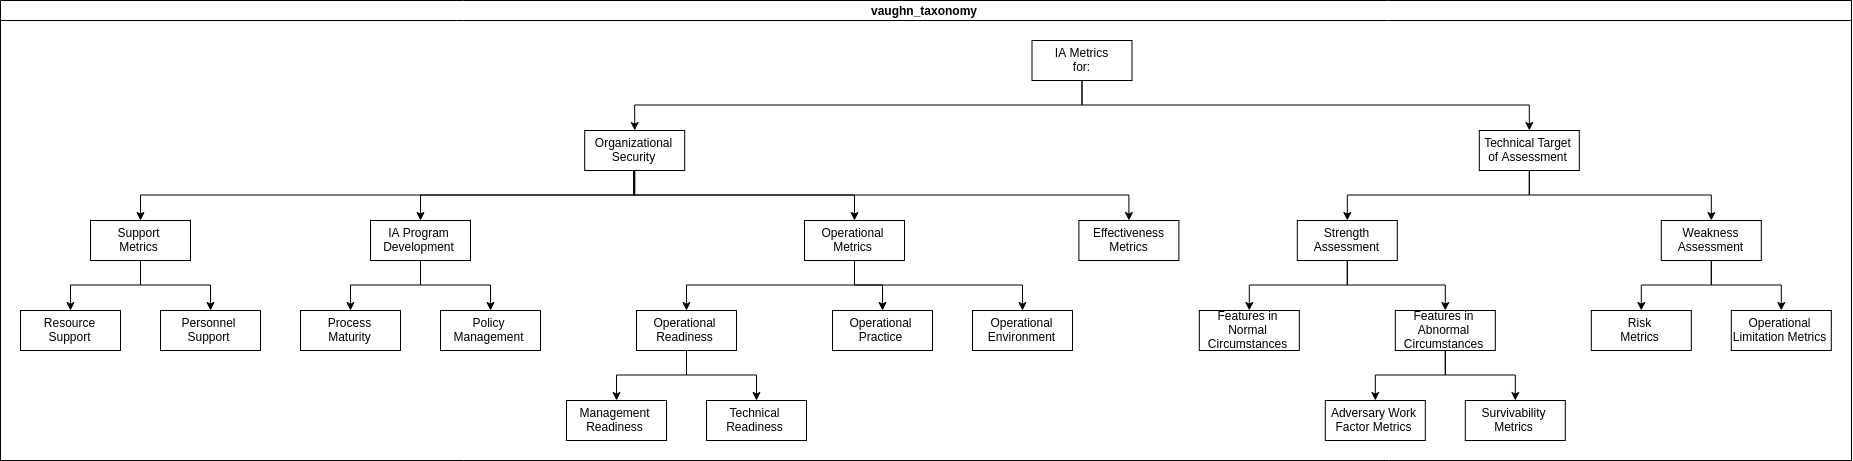
\includegraphics[width=.95\linewidth]{resource/img/ch_background/cybok_metrics/vaughn_taxonomy.png}
\caption{Vaughn's Security Metric Taxonomy\cite{Vaughn_Henning_Siraj_2003}}
\label{fig:background:vaughn_taxonomy}
\end{figure} 

Vaughn’s taxonomy\cite{Vaughn_Henning_Siraj_2003} from 2003 is heavily influenced by federal, and in particular defense department, perspectives on information assurance metrics. The classification tree is heavy on the side of personnel and regulatory metrics compared to other surveys, and the categories draw from military concepts of operational readiness, threat identification, and target acquisition. The survey makes some important observations about properties common to all security metrics. These are presented as binary values which may not be suitable for all metrics, but establishes universal metric attributes we can use in any system.


\begin{figure}[ht]
\centering
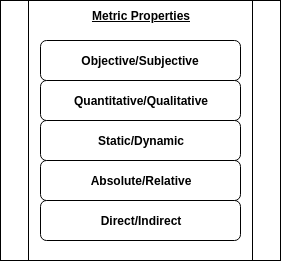
\includegraphics[width=.35\linewidth]{resource/img/ch_background/cybok_metrics/vaughn_metric_propertie.png}
\caption{Vaughn's metric properties\cite{Vaughn_Henning_Siraj_2003}}
\label{fig:background:vaughn_metric_props}
\end{figure} 



\begin{figure}[ht]
\centering
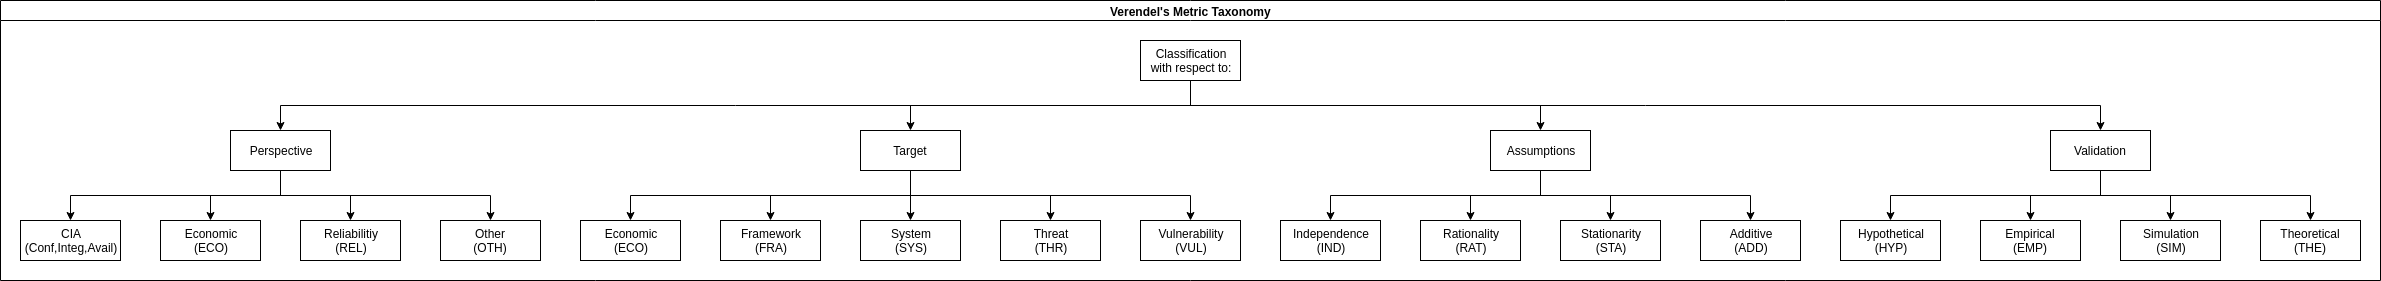
\includegraphics[width=.95\linewidth]{resource/img/ch_background/cybok_metrics/verendel_model_taxonomy.png}
\caption{Verendel's Security Metric Taxonomy \cite{Verendel_2009}}
\label{fig:background:verendel_taxonomy}
\end{figure} 

Verendel’s survey\cite{Verendel_2009} is a critical analysis of the claim that security is quantifiable. The premise is that most of the published models and metrics that attempt to measure security lack the scientific rigor to corroborate or validate their hypothesis. 
The scope of \cite{Verendel_2009} is limited to operational security measurements and assumes measurement primitives include systems, threats, and vulnerabilities.
90 sources published between 1981 and 2008 were surveyed (down selected from 140). These 90 sources are then classified on 4 properties: 
\begin{itemize}
\item \textbf{Perspective}: describes the approach taken to security. { CIA, ECO, REL, OTH}
\item \textbf{Target}: what the source attempts to quantify.{ECO, FRA, SYS, THR, VUL}
\item \textbf{Assumptions}: assumptions made by the source: {IND, RAT, STA, ADD}
\item \textbf{Validation}: how the source supported findings: {HYP, EMP, SIM, THE}
\end{itemize}

Verendel shows that some classes of metrics, specifically cryptographic strength and intrusion detection performance, are validated frequently in the literature through commonly understood methods, while the remaining metric classes are insufficiently validated. 

\begin{figure}[ht]
\centering
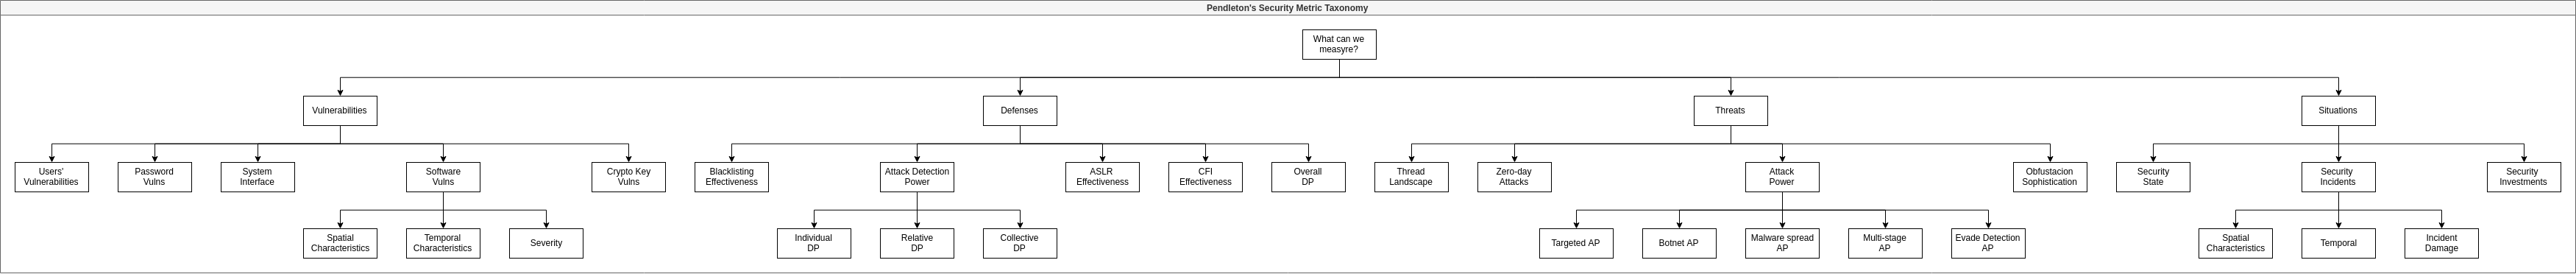
\includegraphics[width=.95\linewidth]{resource/img/ch_background/cybok_metrics/pendleton_metric_taxonomy_drawio.png}
\caption{Pendleton's Security Metric Taxonomy\cite{Pendleton_Garcia-Lebron_Cho_Xu_2016}}
\label{fig:background:pendleton_taxonomy}
\end{figure} 


Pendleton’s survey\cite{ Pendleton_Garcia-Lebron_Xu_2016, Pendleton_Garcia-Lebron_Cho_Xu_2016} approach focuses on metrics that quantify attack and defense interactions. Metrics from 158 sources are classified as measuring one or more of Vulnerabilities, Threats, Defenses, Situations. Situations in this case is a comprehensive metric, with Pendleton’s example subgroups measuring security state over time, successful attacks over time (incident rate), and return on economic investment. Select metrics aligned with Pendleton's survey are shown in Table \ref{tab:pendleton_metrics}.

% \begin{longtable}{@{}llllll@{}}
\begin{tiny}
 \begin{longtable}{@{}|p{0.2\linewidth}|p{0.5\linewidth}|p{0.3\linewidth}|@{}}
% \begin{longtable}{@{}lll@{}}
\toprule
Measuring what? & Representative Metrics Systemized in Paper & Desirable Security Metrics \\* \midrule
\endhead
%
 \multicolumn{3}{c}{\textbf{Measuring System Vulnerabilities}} \\* \midrule
users’ vulnerabilities & user’s susceptibility to phishing attacks \cite{Sheng_Holbrook_Kumaraguru_Cranor_Downs_2010}, user’s susceptibility to malware infection \cite{levesque2013a} & user’s susceptibility to class(es) of attacks (e.g., social-engineering) \\
password vulnerabilities & parameterized/statistical password guessability  \cite{Weir_Aggarwal_Collins_Stern_2010, Bonneau_2012a, Kelley_Komanduri_Mazurek_Shay_Vidas_Bauer_Christin_Cranor_Lopez, Ur_Segreti_Bauer_Christin_Cranor_Komanduri_Kurilova_Mazurek_Melicher_Shay} & worst-case and average-case parameterized\cite{Bonneau_2012b} \\
 &   password entropy\cite{Burr_Dodson_Polk_2006} & password guessability \\
system interface & attack surface \cite{Manadhata_Wing_2010}, exercised attack-surface\cite{Nayak_Marino_Efstathopoulos_Dumitras_2014} & interface-induced susceptibility \\
software vulnerabilities & unpatched vulnerabilities\cite{Chew_Swanson_Stine_Bartol_Brown_Robinson_2008}, exploited vulnerabilities \cite{Nayak_Marino_Efstathopoulos_Dumitras_2014}, vulnerability prevalence \cite{Zhang_Durumeric_Bailey_Liu_Karir_2014} &  \\
vulnerability spatial characteristics &  & vulnerability situation awareness \\
vulnerability temporal characteristics & historical (exploited) vulnerability\cite{Al-Shaer_Khan_Ahmed_2008, Ahmed_Al-Shaer_Khan_2008} , future (exploited) vulnerability \cite{Al-Shaer_Khan_Ahmed_2008, Ahmed_Al-Shaer_Khan_2008}, tendency-to-be-exploited \cite{Sabottke_Suciu_Dumitras}, vulnerability life-time \cite{Frei_Feb_2010, Nappa_Johnson_Bilge_Caballero_Dumitras_2015, Yilek_Rescorla_Shacham_Enright_Savage_2009, durumeric2014a, Zhang_Durumeric_Bailey_Liu_Karir_2014}, & vulnerability vector at any time†, distribution of vulnerability lifetime \\
vulnerability severity & CVSS score {[}of Incident Response and (FIRST) {]}, availability of exploit \cite{Bilge_Dumitras_2012}  & patching priority† , global damage \\
cryptographic key vulnerabilities & vulnerable cryptographic keys \cite{Yilek_Rescorla_Shacham_Enright_Savage_2009, durumeric2014a} Heninger et al. 2012 & (avoidable via prudential engineering) \\* \midrule
 \multicolumn{3}{c}{\textbf{Measuring Defenses} } \\* \midrule
effectiveness of blacklisting & reaction time  \cite{Kuhrer_Rossow_Holz_2014} coverage\cite{Kuhrer_Rossow_Holz_2014}  & blacklisting probability  \\
attack detection power &  &  \\
individual detection power & detection time\cite{Rajab_Monrose_Terzis_2005}, false-positive, false-negative, true-positive, true-negative, ROC, intrusion & detection probability \\
 & detection capability\cite{Gu_Cardenas_Lee_2008}, cost\cite{Gaffney} &  \\
relative detection power & relative effectiveness\cite{Boggs_Stolfo_2011, Boggs_Du_Stolfo_2014} & relative effectiveness against unknown attacks \\
collective detection power & collective effectiveness \cite{Boggs_Stolfo_2011, Morales_Xu_Sandhu_2012, Boggs_Du_Stolfo_2014, Mohaisen_Alrawi_2014, Yardon_2014}& collective effectiveness against unknown attacks \\
ASLR effectiveness & entropy \cite{Shacham_Page_Pfaff_Goh_Modadugu_Boneh_2004}, effective entropy\cite{Herlands_Hobson_Donovan_2014} & security gain†, extra attack effort† \\
CFI effectiveness & CFG accuracy {[}Evans et al. 2015{]}, & CFI resilience† , CFI power  \\
overall defense power & penetration resistance\cite{Levin_2003}, indirect MTD effectiveness\cite{Han_Lu_Xu_2014}& resistance against unknown attacks†, direct MTD effectiveness \\* \midrule
 \multicolumn{3}{c}{\textbf{Measuring Threats}} \\* \midrule
threat landscape & exploit kits {[}Ablon et al. 2014{]}, malicious network\cite{Zhang_Zhang_Ou_2014}, rogue network & comprehensive cyber threat posture \\
 &\cite{Stone-Gross_Kruegel_Almeroth_Moser_Kirda_2009}, ISP badness \cite{Johnson_Chuang_Grossklags_Christin_2012} control-plan reputation\cite{Konte_Perdisci_Feamster_2015}, early-detection time\cite{Konte_Perdisci_Feamster_2015}, cybersecurity posture\cite{Zhan_Xu_Xu_2015}, sweep-time\cite{Zhan_Xu_Xu_2015}, attackrate \cite{Zhan_Xu_Xu_2015} &  \\
zero-day attacks & number of zero-day attacks {[}Corporation 2012{]}, lifetime of zero-day attacks\cite{Bilge_Dumitras_2012}, number of zero-day attack victims \cite{Bilge_Dumitras_2012}& susceptibility of a computer to zero-day attacks \\
attack power &  &  \\
power of targeted attacks & targeted threat index\cite{Hardy_Crete-Nishihata_Kleemola_Senft_Sonne_Wiseman_Gill_Deibert_2014} & susceptibility to targeted attacks \\
power of botnet & botnet size\cite{Dagon_Zou_Lee_2006}, botnet efficiency\cite{Dagon_Gu_Lee_Lee_2007}, botnet robustness\cite{Dagon_Gu_Lee_Lee_2007} & botnet attack power, botnet resilience with counter-countermeasures \\
power of malware spreading & infection rate\cite{Chen_Ji_2007} & attack power , wasted scans \\
power of multi-stage attacks & necessary defense\cite{Sheyner_Haines_Jha_Lippmann_Wing_2002}, weakest adversary\cite{Pamula_Jajodia_Ammann_Swarup_2006}, attack paths & multi-stage attack power \\
 & \cite{Ritchey_Ammann_2000,  Sheyner_Haines_Jha_Lippmann_Wing_2002, Jha_Sheyner_Wing_2002, Cheng_Deng_Li_DeLoach_Singhal_Ou_2014}, k-zero-day-safety &  \\
 & \cite{Wang_Jajodia_Singhal_Noel_2010}, effort-to-security-failure\cite{Dacier_Deswarte_Kaaniche, Ortalo_1999} &  \\
power of evading detection & (no nontrivial metrics defined) & evasion capability \\
obfuscation sophistication & obfuscation prevalence\cite{Roundy_Miller_2013}, packer structural complexity\cite{Ugarte-Pedrero_Balzarotti_Santos_Bringas_2015} & obfuscation sophistication \\* \midrule
 \multicolumn{3}{c}{\textbf{Measuring Situations}} \\* \midrule
security state & fractions of compromised computers at time t, probability a computer is compromised at time t\cite{LeMay_Ford_Keefe_Sanders_Muehrcke_2011, Da_Xu_Xu_2014, Xu_2014a} & S(t) and si (t) for any security incidents   \\
incident spatial characteristics & incident rate \cite{Microsoft_2013, Yen_Heorhiadi_Oprea_Reiter_Juels_2014, levesque2013a}; Maier et al., & incident occurrence frequency \\
 & encounter rate\cite{Yen_Heorhiadi_Oprea_Reiter_Juels_2014,Mezzour_Carley_Carley_2015, Microsoft_2013,levesque2013a} &  \\
incident temporal characteristics & delay in incident detection {[}for Internet Security 2010{]}, time between incidents {[}for Internet Security 2010; & predictive incident occurrence frequency† \\
 & \cite{Jonsson_Olovsson_1997, Madan_Gogeva-Popstojanova_Vaidyanathan_Trivedi_2002, Holm_2014}, time-to-first-compromise &  \\
 & \cite{Jonsson_Olovsson_1997,Madan_Gogeva-Popstojanova_Vaidyanathan_Trivedi_2002,Holm_2014} &  \\
incident damage & cost of incidents {[}for Internet Security 2010{]} & predictive incident damage† \\
security investments & security spending\cite{Chew_Swanson_Stine_Bartol_Brown_Robinson_2008}, security budget {[}for Internet Security 2010{]} & payoff of security investment \\* \bottomrule
\caption{Pendleton's Survey: Selected Attack \& Defense Metrics\cite{Pendleton_Garcia-Lebron_Cho_Xu_2016}}
\label{tab:pendleton_metrics}\\
\end{longtable}
\end{tiny}

In the conclusions Pendleton hints at some properties desirable in all security metrics (additivity) but stops short of declaring these necessary traits for validation, or even enumerating the full list of common metric attributes. 


\begin{figure}[ht]
\centering
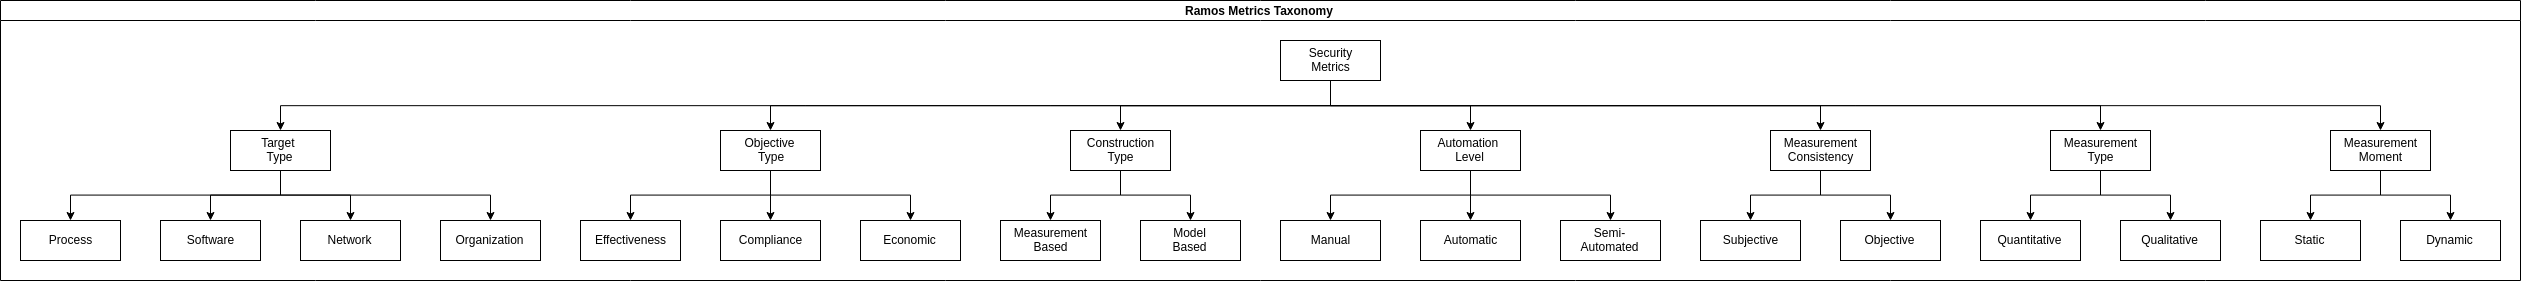
\includegraphics[width=.95\linewidth]{resource/img/ch_background/cybok_metrics/ramos_taxonomy.png}
\caption{Ramos' Security Metric Taxonomy\cite{Ramos_Lazar_Filho_Rodrigues_2017}}
\label{fig:background:ramos_taxonomy}
\end{figure} 

Ramos\cite{Ramos_Lazar_Filho_Rodrigues_2017} focuses on model-based network security metrics exclusively, and provides a list of 5 properties distinct from Vaughn’s in \cite{Vaughn_Henning_Siraj_2003} which all good metrics should possess. Again we see validation listed as necessary to all types of metrics. Ramos cites 146 sources in the survey and consolidates classification to around 75 distinct metrics.

\begin{figure}[ht]
\centering
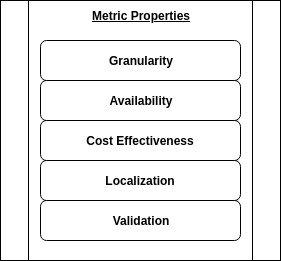
\includegraphics[width=.35\linewidth]{resource/img/ch_background/cybok_metrics/ramos_metric_properties.png}
\caption{Ramos’ Model Based Security Metric Properties\cite{Ramos_Lazar_Filho_Rodrigues_2017}}
\label{fig:background:ramos_metric_props}
\end{figure} 

The primary classification in \cite{Ramos_Lazar_Filho_Rodrigues_2017} is by target. A metric can evaluate a Process (eg SSE-CMM), Software, the Network, or the Organization - which includes physical and personnel security metrics. The Construction Type category distinguishes between empirical and analytical metrics, the latter requiring some type of model (attack graph, markov, etc)  to perform evaluation. Measurement Consistency describes whether a metric is objective or subjective. 

Ramos splits the set of model based quantitative security metrics into 3 buckets based on the input model the metric expects (Stochastic, Graph, Other) with other including attack nets, petri nets, etc. This partitioning is likely to make reporting results easier as, in our experience, these input models will be produced from the same set of input data. Should we consider a metric that computes a function analytically and another that estimates the same quantity through simulation separate metrics? In table IX\cite{Ramos_Lazar_Filho_Rodrigues_2017} Ramos indicates the lack of validation across the surveyed metrics even when the author’s own inline validation we accounted for. Select metrics aligned with Ramos' survey are shown in Table \ref{tab:ramos_metrics}.


\begin{tiny}
\begin{longtable}{@{}lllll@{}}
\toprule
\textbf{Metric} & \textbf{Compliance} & \textbf{Moment} & \textbf{Consistency} &  \\ \midrule
\endhead
%
\bottomrule
\endfoot
%
\endlastfoot
%

MTTF \cite{Dacier_Deswarte_Kaaniche_1996a}\cite{Dacier_Deswarte_Kaaniche} & compliance & dynamic & objective &  \\
METF \cite{Ortalo_1999} & compliance & dynamic & subjective &  \\
MTSF \cite{Almasizadeh_Azgomi_2013a}, \cite{Almasizadeh_Azgomi_2009}, \cite{Almasizadeh_2009} & compliance & static & subjective &  \\
MTFF \cite{Al-Kuwaiti_Kyriakopoulos_Hussein_2009}, \cite{Sallhammar_2006} & compliance & static & subjective &  \\
MTTC by McQueen et al. \cite{McQueen_Boyer_Flynn_Beitel_2005} & compliance & static & subjective &  \\
MTTC by Leversage et al. \cite{Leversage_Byres_2008} & compliance & static & subjective &  \\
Steady-State Security \cite{Almasizadeh_Azgomi_2013a}, \cite{Almasizadeh_Azgomi_2009}, \cite{Almasizadeh_2009} & non-compliance & static & subjective &  \\
Reliability \cite{Jha_Sheyner_Wing_2002} & compliance & static & objective &  \\
Success Likelihood \cite{Kanoun_Dubus_Papillon_Cuppens_Boulahia_Cuppens_2012} & non-compliance & dynamic & subjective &  \\
q \cite{Li_Parker_Xu_2011} & non-compliance & static & objective &  \\
Shortest Path \cite{Phillips_Swiler_1998}, \cite{Idika_Bhargava_2012} & compliance & dynamic & objective &  \\
Number of Paths \cite{Ortalo_1999}, \cite{Idika_Bhargava_2012} & non-compliance & dynamic & objective &  \\
Mean of Path Lengths \cite{Li_Vaughn_2006}, \cite{Idika_Bhargava_2012} & compliance & dynamic & objective &  \\
Normalized Mean of Path Lengths\cite{Idika_Bhargava_2012} & compliance & dynamic & objective &  \\
Assistive metrics: SDPL, MoPL, MePL \cite{Idika_Bhargava_2012} & compliance & dynamic & objective &  \\
Weakest Adversary \cite{Pamula_Jajodia_Ammann_Swarup_2006} & compliance & static &  subjective & \\
Network Compromise Percentage \cite{Lippmann_2006} &  non-compliance &  dynamic &  objective &  \\
Network Compromise Percentage \cite{Lippmann_2006} & non-compliance &  dynamic &  objective & \\
State Rank \cite{Mehta_Bartzis_Zhu_Clarke_Wing_2006} & non-compliance & static & subjective &  \\
Cumulative Score \cite{Noel_Jajodia} & non-compliance & static & objective &  \\
AGP \cite{Wang_Islam_Long_Singhal_Jajodia_2008} & non-compliance & static & subjective &  \\
Attack Resistance \cite{Wang_Singhal_Jajodia_2007a} & compliance & static & subjective &  \\
Enhanced Cumulative Score \cite{Homer_Zhang_Ou_Schmidt_Du_Rajagopalan_Singhal_2013} & non-compliance & static & subjective &  \\
Liu and Man’s metric \cite{Liu_Man_2005} & non-compliance & dynamic & subjective &  \\
Frigault and Wang’s metric \cite{Frigault_Wang_2008} & non-compliance & static & subjective &  \\
Frigault and colleagues’ metric \cite{Frigault_Wang_Singhal_Jajodia_2008} & non-compliance & dynamic & subjective &  \\
Poolsappasit and colleagues’ metric \cite{Poolsappasit_Dewri_Ray_2012} & non-compliance & dynamic & subjective &  \\
Xie and colleagues’ metric \cite{Xie_Li_Ou_Liu_Levy_2010} & non-compliance & dynamic & subjective &  \\
Dantu and colleagues’ metric \cite{Dantu_Kolan_Cangussu_2009}, \cite{Dantu_Kolan_2005}, \cite{Dantu_Loper_Kolan_2004} & non-compliance & dynamic & subjective &  \\
Expected Difficulty \cite{Ghosh_Bhattacharya_2012} & compliance & static & subjective &  \\
VEA-bility \cite{Tupper_Zincir-Heywood_2008} & compliance & static & subjective &  \\
k-zero day safety \cite{Wang_Jajodia_Singhal_Cheng_Noel_2014}, \cite{Wang_Jajodia_Singhal_Noel_2010} & compliance & static & subjective &  \\
d2-Diversity (least attacking effort) \cite{Zhang_Wang_Jajodia_Singhal_Albanese_2016}, \cite{Wang_Zhang_Jajodia_Singhal_Albanese_2014} & compliance & static & subjective &  \\
d3-Diversity (avg. attacking effort) \cite{Zhang_Wang_Jajodia_Singhal_Albanese_2016}, \cite{Wang_Zhang_Jajodia_Singhal_Albanese_2014} & non-compliance & static & subjective &  \\
d1-Diversity (\% of distinct resources) \cite{Zhang_Wang_Jajodia_Singhal_Albanese_2016}, \cite{Wang_Zhang_Jajodia_Singhal_Albanese_2014} & compliance & static & subjective &  \\
Seclius \cite{Zonouz_Berthier_Khurana_Sanders_Yardley_2015} & non-compliance & dynamic & objective &  \\
Damage risk \cite{Chatzipoulidis_Michalopoulos_Mavridis_2015} & non-compliance & static & subjective &  \\
Mean Privacy \cite{Almasizadeh_Azgomi_2013a} & non-compliance & static & subjective &  \\
Security Meter \cite{Sahinoglu_2005}, \cite{Sahinoglu_2008} & non-compliance & static & subjective &  \\
Policy Security Score \cite{Abedin_Nessa_Al-Shaer_Khan_2006} & compliance & dynamic & subjective &  \\
Probabilistic Vulnerability Measure \cite{Ahmed_Al-Shaer_Khan_2008} & non-compliance & dynamic & subjective &  \\
Attack Propagation \cite{Ahmed_Al-Shaer_Taibah_Khan_2011} & non-compliance & dynamic & subjective &  \\
ADVISE \cite{LeMay_Ford_Keefe_Sanders_Muehrcke_2011} & compliance & static & subjective &  \\* \bottomrule
\caption{Ramos' Survey: Selected Model Based Security Metrics\cite{Ramos_Lazar_Filho_Rodrigues_2017}}
\label{tab:ramos_metrics}\\
\end{longtable}
\end{tiny}


\begin{figure}[ht]
\centering
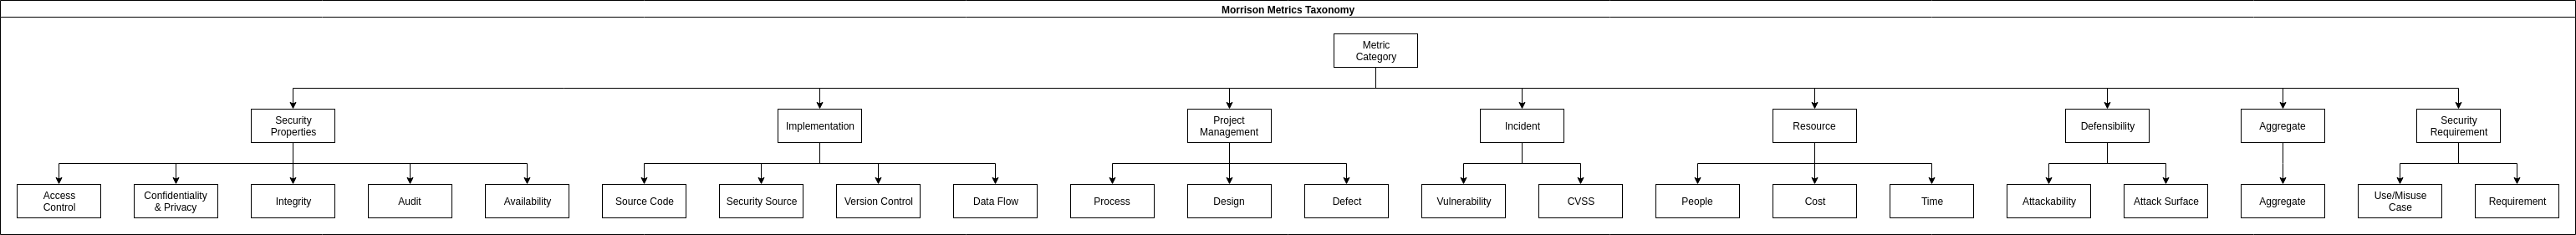
\includegraphics[width=.95\linewidth]{resource/img/ch_background/cybok_metrics/morrison_taxonomy.png}
\caption{Morrison's Security Metric Taxonomy\cite{Morrison_Moye_Pandita_Williams_2018}
\label{fig:background:morrison_taxonomy}}
\end{figure} 

Morrison surveys 71 sources (down selected from 4818) to classify 324 security metrics from the SDLC. The number of metrics for each group are summarized in table \ref{fig:background:morrison_metric_props}.

\begin{tiny}
% \begin{longtable}{@{}llllll@{}}
 \begin{longtable}{@{}p{0.25\linewidth}p{0.15\linewidth}p{0.05\linewidth}p{0.1\linewidth}p{0.1\linewidth}p{0.1\linewidth}@{}}
\cmidrule(r){1-6}
\textit{\textbf{Metric Name}} & \textit{\textbf{Category}} & \textbf{Paper} & \textbf{Method} & \textbf{Scale} & \textbf{Phase} \\* \cmidrule(r){1-6}
\endhead
%
Mechanism strength & Design  & \cite{Liu_Man_2005} & Quantitative & count & Implementation \\
Action Register & Access Control  & \cite{Villarrubia_Fernandez-Medina_Piattini_2006} & Qualitative & count & Operations \\
Alphabet Size & Access Control  & \cite{Villarrubia_Fernandez-Medina_Piattini_2006} & Qualitative & Enumeration & Operations \\
Authentication Period & Access Control  & \cite{Villarrubia_Fernandez-Medina_Piattini_2006} & Qualitative & Enumeration & Operations \\
Block by User Cancellation & Access Control  & \cite{Villarrubia_Fernandez-Medina_Piattini_2006} & Qualitative & ordinal & Operations \\
Group Password & Access Control  & \cite{Villarrubia_Fernandez-Medina_Piattini_2006} & Quantitative & count & Operations \\
Information about Use & Access Control  & \cite{Villarrubia_Fernandez-Medina_Piattini_2006} & Qualitative & Enumeration & Operations \\
Initial Communication & Access Control  & \cite{Villarrubia_Fernandez-Medina_Piattini_2006} & Quantitative & duration & Operations \\
Input Visualization & Access Control  & \cite{Villarrubia_Fernandez-Medina_Piattini_2006} & Qualitative & Enumeration & Operations \\
Maximum Life Time & Access Control  & \cite{Villarrubia_Fernandez-Medina_Piattini_2006} &  & Not specified & Implementation \\
Maximum Number of Erroneous Attempts & Access Control  & \cite{Villarrubia_Fernandez-Medina_Piattini_2006} & Qualitative & ordinal & Operations \\
Minimum Length & Access Control  & \cite{Villarrubia_Fernandez-Medina_Piattini_2006} & Qualitative & ordinal & Operations \\
Minimum Life Time & Access Control  & \cite{Villarrubia_Fernandez-Medina_Piattini_2006} &  & Not specified & Operations \\
Net Transmission & Access Control  & \cite{Villarrubia_Fernandez-Medina_Piattini_2006} & Qualitative & Enumeration & Operations \\
Number of Different Classes & Access Control  & \cite{Villarrubia_Fernandez-Medina_Piattini_2006} &  & Not specified & Operations \\
Password Reassigning & Access Control  & \cite{Villarrubia_Fernandez-Medina_Piattini_2006} & Quantitative & Time & Operations \\
Predefined Users & Access Control  & \cite{Villarrubia_Fernandez-Medina_Piattini_2006} & Qualitative & ordinal & Operations \\
Record Length & Access Control  & \cite{Villarrubia_Fernandez-Medina_Piattini_2006} & Qualitative & ordinal & Operations \\
Selection Restriction & Access Control  & \cite{Villarrubia_Fernandez-Medina_Piattini_2006} & Qualitative & ordinal & Operations \\
Source Selection & Access Control  & \cite{Villarrubia_Fernandez-Medina_Piattini_2006} & Qualitative & ordinal & Operations \\
Storage Class & Confidentiality and Privacy  & \cite{Villarrubia_Fernandez-Medina_Piattini_2006} & Qualitative & Enumeration & Operations \\
User Identificator & Access Control  & \cite{Villarrubia_Fernandez-Medina_Piattini_2006} &  & Not specified & Operations \\
User Training & Access Control  & \cite{Villarrubia_Fernandez-Medina_Piattini_2006} & Quantitative & duration & Operations \\
CVSS Score & CVSS  & \cite{Schryen_Kadura_2009} & Quantitative & count & Operations \\
Patch Index & Vulnerability  & \cite{Schryen_Kadura_2009} & Quantitative & count & Operations \\
Annual Loss Expectancy (ALE) & Cost  & \cite{Bohme_Felegyhazi_2010} & Quantitative & duration & Operations \\
Return on Penetration Testing & Cost  & \cite{Bohme_Felegyhazi_2010} & Qualitative & ordinal & Operations \\
Business Adjusted Risk & Cost  & \cite{Trcek_2010} & Quantitative & count & Operations \\
Daily Vulnerability Exposure & Vulnerability  & \cite{Trcek_2010} & Qualitative & ordinal & Operations \\
Vulnerability Index & Vulnerability  & \cite{Trcek_2010} & Qualitative & ordinal & Operations \\
CN Betweenness & People  & \cite{Meneely_Williams_2010} & Quantitative & count & Operations \\
DN Max Edge Betweenness & People  & \cite{Meneely_Williams_2010} & Quantitative & Time & Operations \\
Num Commits & Version Control  & \cite{Meneely_Williams_2010} & Quantitative & Not specified & Operations \\
NumDevs & People  & \cite{Meneely_Williams_2010} & Qualitative & ordinal & Operations \\
Vulnerability & Vulnerability  & \cite{Meneely_Williams_2010} & Qualitative & ordinal & Operations \\
Contributions & Version Control  & \cite{Perl_Dechand_Smith_Arp_Yamaguchi_Rieck_Fahl_Acar_2015} & Qualitative & ordinal & Operations \\
Fork count & Version Control  & \cite{Perl_Dechand_Smith_Arp_Yamaguchi_Rieck_Fahl_Acar_2015} &  & Not specified & Operations \\
Number of commits & Version Control  & \cite{Perl_Dechand_Smith_Arp_Yamaguchi_Rieck_Fahl_Acar_2015} & Qualitative & ordinal & Operations \\
Number of hunks & Version Control  & \cite{Perl_Dechand_Smith_Arp_Yamaguchi_Rieck_Fahl_Acar_2015} & Qualitative & ordinal & Operations \\
Patch & Version Control  & \cite{Perl_Dechand_Smith_Arp_Yamaguchi_Rieck_Fahl_Acar_2015} & Quantitative &  & Operations \\
Patch keywords & Version Control  & \cite{Perl_Dechand_Smith_Arp_Yamaguchi_Rieck_Fahl_Acar_2015} & Quantitative & count & Operations \\
Programming language & Source Code  & \cite{Perl_Dechand_Smith_Arp_Yamaguchi_Rieck_Fahl_Acar_2015} & Qualitative & currency & Operations \\
Star count & Version Control  & \cite{Perl_Dechand_Smith_Arp_Yamaguchi_Rieck_Fahl_Acar_2015} & Quantitative & ratio & Operations \\
Vulnerability & Vulnerability  & \cite{Perl_Dechand_Smith_Arp_Yamaguchi_Rieck_Fahl_Acar_2015} & Qualitative & currency & Testing \\
Probability Compromised and Repaired (PC) & Attackability & \cite{Marconato_Kaaniche_Nicomette_2013} &  & count & Operations \\
Probability Compromised Not Repaired (PCNR) & Attackability & \cite{Marconato_Kaaniche_Nicomette_2013} & Quantitative & Classes & Design \\
Probability Secure (PS) & Attackability & \cite{Marconato_Kaaniche_Nicomette_2013} & Quantitative & probability & All \\
Probability Unpatched Compromise (PPC) & Attackability & \cite{Marconato_Kaaniche_Nicomette_2013} & Quantitative & ratio & Design \\
Vulnerability Disclosure & Vulnerability  & \cite{Marconato_Kaaniche_Nicomette_2013} &  & probability & Operations \\
Vulnerability Discovery & Vulnerability  & \cite{Marconato_Kaaniche_Nicomette_2013} &  & count & Operations \\
Vulnerability Patch & Vulnerability  & \cite{Marconato_Kaaniche_Nicomette_2013} &  & count & Operations \\
Access Complexity (AC) & CVSS  & \cite{Scarfone_Mell_2008} &  & count & Operations \\
Access Vector (AV) & CVSS  & \cite{Scarfone_Mell_2008} & Quantitative & Classes & Design \\
Authentication (AU) & CVSS  & \cite{Scarfone_Mell_2008} &  & probability & Operations \\
Availability Impact (A) & CVSS  & \cite{Scarfone_Mell_2008} & Quantitative & Ratio & Requirements \\
Availability Requirement (AR) & CVSS  & \cite{Scarfone_Mell_2008} & Quantitative & probability & Operations \\
Collateral Damage Potential (CDP) & CVSS  & \cite{Scarfone_Mell_2008} & Quantitative & probability & Operations \\
Confidentiality Impact (C) & CVSS  & \cite{Scarfone_Mell_2008} & Quantitative & probability & Operations \\
Confidentiality Requirement (CR) & CVSS  & \cite{Scarfone_Mell_2008} & Quantitative & probability & Operations \\
Exploitability (TE) & CVSS  & \cite{Scarfone_Mell_2008} & Quantitative & count & Design \\
Integrity Impact (I) & CVSS  & \cite{Scarfone_Mell_2008} &  & count & Operations \\
Integrity Requirement (IR) & CVSS  & \cite{Scarfone_Mell_2008} & Quantitative & count & Operations \\
Remediation Level (RL) & CVSS  & \cite{Scarfone_Mell_2008} & Quantitative & count & Operations \\
Report Confidence (RC) & CVSS  & \cite{Scarfone_Mell_2008} & Quantitative & count & Operations \\*
\caption{Morrison's Survey: Selected Software Security Metrics\cite{Morrison_Moye_Pandita_Williams_2018}}
\label{tab:morrison_metrics}\\
\end{longtable}
\end{tiny}


\begin{figure}[ht]
\centering
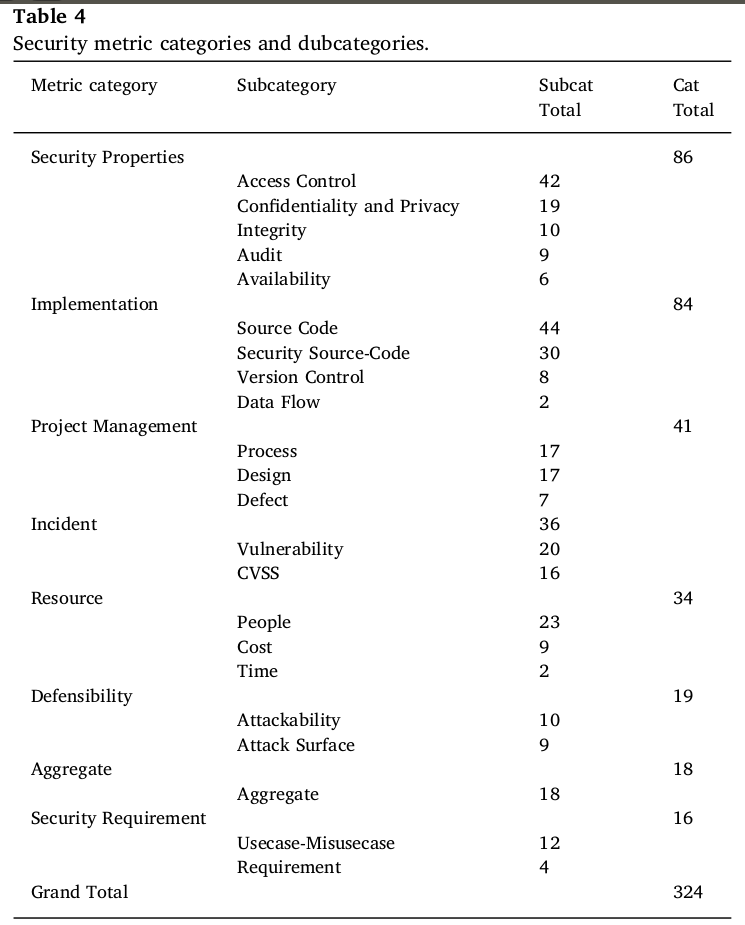
\includegraphics[width=.55\linewidth]{resource/img/ch_background/cybok_metrics/morrison_metric_props_table.png}
\caption{\# Security Metrics by Category/SubCategory (out of 324)\cite{Morrison_Moye_Pandita_Williams_2018}
\label{fig:background:morrison_metric_props}}
\end{figure} 

As these metrics are focused on software security, Morrison finds that many are either normalized to existing software metrics or are extensions thereof. Subcategories of Security Properties seem to be based on surveys about the listed property but this may reflect the source authors rather than an inability to automate collection. Incident Metrics more closely map to previous other’s Vulnerabilities categories as nothing indicates successful attacks are being examined here. 
From the paper’s findings, 85\% of metrics surveyed have only been proposed and evaluated by the author, pointing again to the need for metric validation. Very few metrics apply to design time or test time evaluation in the SDLC - most are tuned for production deployment. The majority of metrics are subjective, relying on user feedback. Select metrics aligned with Morrison's survey are shown in Table \ref{tab:morrison_metrics}.



\subsection{Security Metrics Taxonomy}\label{sec:background:metrics_by_cybok}


Above we reviewed some existing classification methods for security metrics. These included taxonomies from both narrow and broadly focused surveys. While there is certainly overlap within some of the categories and properties identified, there is also collision between similar sounding concepts from different sources. To remove ambiguity, and more importantly to address the immediate question, we can map all our security metrics onto the taxonomy derived from the Cyber Security Body of Knowledge. The CyBoK is an effort to collect and maintain canonical research across the entirety of the cyber security domain. Included in this mandate is keeping all of it organized, so we can presume that if there is a topic in security we would like to measure, then there will be a corresponding topic in the CyBoK to consult. 

Security metrics can be categorized by the area of cyber security to which they apply. In this respect, the security metric surveys available in recent literature are by nature focused narrowly on a specific subfield, such as cryptographic or software development lifecycle security metrics. To remove ambiguity in terms among surveys, we attempt to include these in a \textit{big-picture} view of the field of cyber security by classifying them under the general headings of the recently released Cyber Security Body of Knowledge\cite{Rashid_Chivers_Danezis_Lupu_Martin} depicted in Figure \ref{fig:intro:cybok}. By grouping our security metrics by Cybok category, we can determine our cyber security metric coverage, and use this context to identify non-security related metrics that would be relevant to the area. 

\subsubsection{Human, Organization, \& Regulatory Metrics}

\begin{figure}[ht]

\begin{mdframed}
\centering
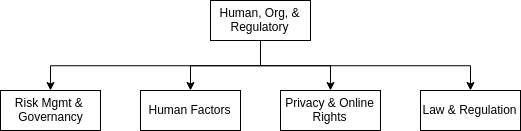
\includegraphics[width=.8\linewidth]{resource/img/ch_background/cybok_metrics/cybok_hor.png}
\end{mdframed}
\caption{Cybok: Human, Organization, \& Regulation Metrics
\label{fig:background:cybok_hor_metrics}}
\end{figure} 

\begin{figure}[ht]
\centering
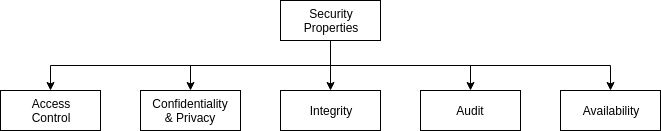
\includegraphics[width=.9\linewidth]{resource/img/ch_background/cybok_metrics/morrison_sec_props.png}
\caption{Most of Morrison’s class for Security Properties would fit under HO\&R.
\label{fig:background:cybok_hor_metrics_morrison}}
\end{figure} 

\begin{figure}[ht]
\centering
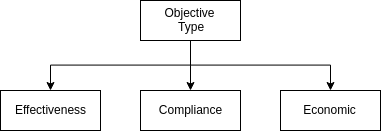
\includegraphics[width=.6\linewidth]{resource/img/ch_background/cybok_metrics/ramos_objective_type.png}
\caption{Ramos’ Objective Type metrics fall under HO\&R (economics is cross cutting).
\label{fig:background:cybok_hor_metrics_ramos}}
\end{figure} 


\begin{figure}[ht]
\centering
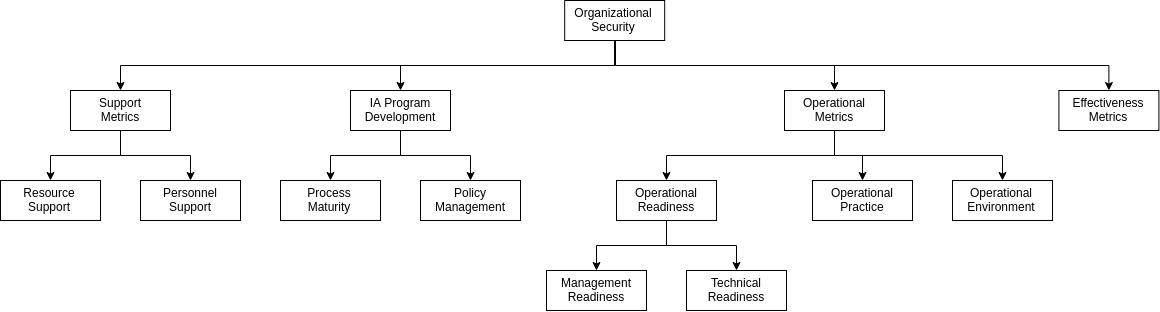
\includegraphics[width=.95\linewidth]{resource/img/ch_background/cybok_metrics/vaughn_org_metrics.png}
\caption{Vaughn’s Organization Security metrics subtree  falls under HO\&R.
\label{fig:background:cybok_hor_metrics_vaughn}}
\end{figure} 

Metrics in HO\&R are usually derived from applicable regulations and policies (ISO, FISMA, HIPPA, PCI, ADA, etc). Often these are counts or ratios that quantify the proportion of assets that are in/out of compliance with the regulation. Typical applications for these metrics are system audits (how many current users have completed mandatory training) or accreditations (how many of these secure operations checkboxes does the current system check).


\subsubsection{Attack \& Defense Metrics}

\begin{figure}[ht]

\begin{mdframed}
\centering
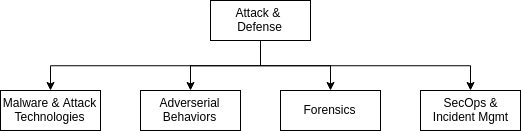
\includegraphics[width=.8\linewidth]{resource/img/ch_background/cybok_metrics/cybok_ad.png}
\end{mdframed}
\caption{Cybok: Attack \& Defense Domain Metrics
\label{fig:background:cybok_ad_metrics}}
\end{figure} 

Attack and defense describes many of the security metrics we have investigated in this thesis. Malware and Attack metrics can quantify an attacker’s capabilities, the DoS’ing bandwidth of a botnet or the number of accounts controlled are examples. Adversarial behaviours might relate to MITRE’s APT and CAPEC attack pattern datasets, but I haven’t encountered metrics that evaluate this yet (although it shows up regularly in threat models). Forensics metrics typically include time to unpack or deobfuscate a malware sample, or the amount of time to determine an indicator of compromise for IDS deployment. SecOps \& Incident Response metrics include standards from the literature such as IDS efficacy and mean time between failures. 

\begin{figure}[ht]
\centering
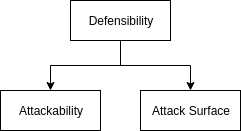
\includegraphics[width=.35\linewidth]{resource/img/ch_background/cybok_metrics/morrison_defensibility.png}
\caption{Morrison’s Defensibility metrics fall generally under A\&D.
\label{fig:background:cybok_ad_morrison}}
\end{figure} 

\begin{figure}[ht]
\centering
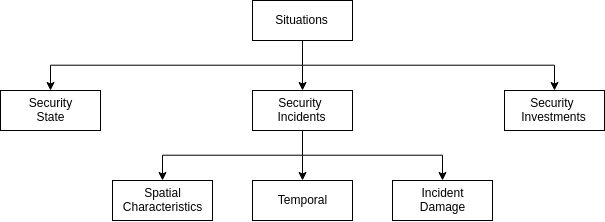
\includegraphics[width=.8\linewidth]{resource/img/ch_background/cybok_metrics/pendleton_situations.png}
\caption{Pendleton’s Situations metrics fall under A\&D.
\label{fig:background:cybok_ad_pendleton}}
\end{figure} 

\begin{figure}[ht]
\centering
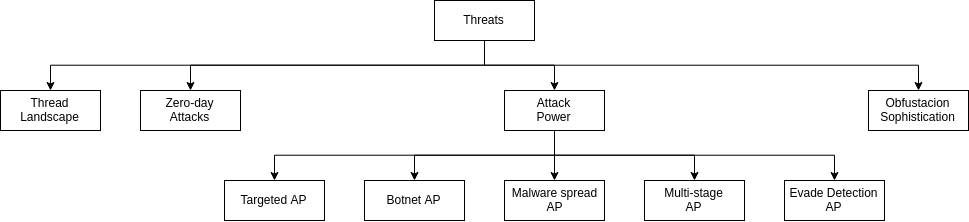
\includegraphics[width=.95\linewidth]{resource/img/ch_background/cybok_metrics/pendleton_threats.png}
\caption{Pendleton’s Threats metrics fall under A\&D.
\label{fig:background:cybok_ad_pendleton_threats}}
\end{figure} 

\begin{figure}[ht]
\centering
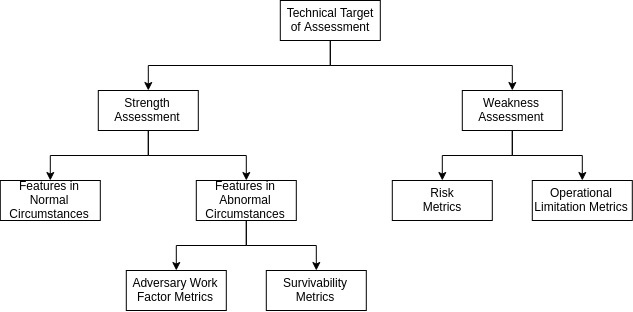
\includegraphics[width=.75\linewidth]{resource/img/ch_background/cybok_metrics/vaughn_ttoa.png}
\caption{Vaughn’s Strength and Weakness metrics fall under A\&D.
\label{fig:background:cybok_ad_vaugh_ttoa}}
\end{figure} 

\subsubsection{Systems Security Metrics}

\begin{figure}[ht]

\begin{mdframed}
\centering
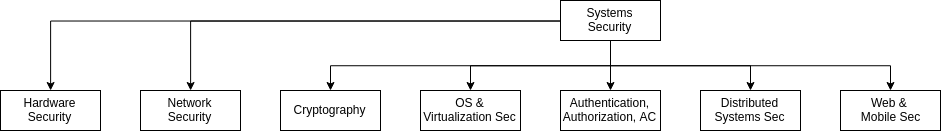
\includegraphics[width=.95\linewidth]{resource/img/ch_background/cybok_metrics/cybok_systems.png}
\end{mdframed}
\caption{Cybok: Systems Domain Metrics
\label{fig:background:cybok_sys_metrics}}
\end{figure} 

Systems security metrics span most aspects of operational security. Hardware and Network security metrics were discussed under infrastructure. Typical applications of cryptographic security metrics include all the formal verification artifacts involved in the validation of a protocol or implementation, along with performance, key size, entropy, etc. OS security metrics may be derived from common criteria/ EAL or measure isolation, weakness to side channels, or number of vulnerabilities known along with severity. 

\begin{figure}[ht]
\centering
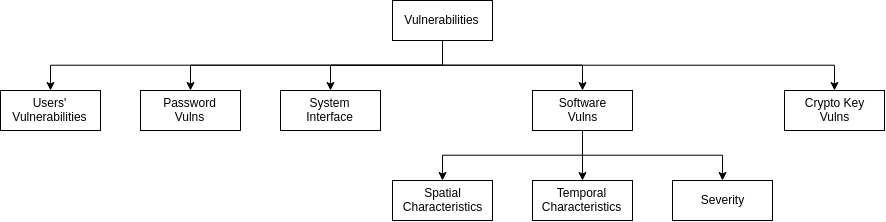
\includegraphics[width=.95\linewidth]{resource/img/ch_background/cybok_metrics/pendleton_vulns.png}
\caption{Pendleton’s Vulnerabilities security metrics fall under System’s security metrics
\label{fig:background:pendleton_vuln_metrics}}
\end{figure} 

Model based network security metrics classified by Ramos\cite{Ramos_Lazar_Filho_Rodrigues_2017} are shown in Figure \ref{fig:background:ramos_taxonomy}. These metrics are designated as Compliance based when a larger value indicates more security. Moment identifies if a measurement can be taken pre-deployment and remains static throughout operation, or if the metric is dynamic and should be measured repeatedly. Consistency distinguishes if the measured value relies on subjective human input or if its evaluation is objective. To compare with network performance metrics like latency or throughput, these security metrics are heavily influenced by subjective criteria. For example, the reliability based models make assumptions about an attacker’s success rate, level of effort, motivations, and capabilities that could change depending on who is filling in the weights. 

% \begin{minipage}{\linewidth}
% % \begin{table}[]
% \resizebox{\textwidth}{!}{%
% \begin{tabular}{@{}lllll@{}}
% \toprule
% \textbf{Metric} & \textbf{Compliance} & \textbf{Moment} & \textbf{Consistency} &  \\ \midrule
% MTTF {[}70{]}, {[}71{]} & compliance & dynamic & objective &  \\
% METF {[}72{]} & compliance & dynamic & subjective &  \\
% MTSF {[}40{]}, {[}73{]}, {[}74{]} & compliance & static & subjective &  \\
% MTFF {[}53{]}, {[}54{]} & compliance & static & subjective &  \\
% MTTC by McQueen et al. {[}8{]}, {[}75{]} & compliance & static & subjective &  \\
% MTTC by Leversage et al. {[}76{]} & compliance & static & subjective &  \\
% Steady-State Security {[}40{]}, {[}73{]}, {[}74{]} & non-compliance & static & subjective &  \\
% Reliability {[}79{]} & compliance & static & objective &  \\
% Success Likelihood {[}80{]} & non-compliance & dynamic & subjective &  \\
% q {[}81{]} & non-compliance & static & objective &  \\
% Shortest Path {[}83{]}, {[}10{]} & compliance & dynamic & objective &  \\ 
% Number of Paths {[}72{]}, {[}10{]} & non-compliance & dynamic & objective &  \\
% Mean of Path Lengths {[}95{]}, {[}10{]} & compliance & dynamic & objective &  \\
% Normalized Mean of Path Lengths {[}10{]} & compliance & dynamic & objective &  \\
% Assistive metrics: SDPL, MoPL, MePL {[}10{]} & compliance & dynamic & objective &  \\
% Weakest Adversary {[}96{]}  & compliance & static & subjective&  \\
% Network Compromise Percentage {[}97{]} & non-compliance &  dynamic &  objective &\\
% State Rank {[}98{]} & non-compliance & static & subjective &  \\
% Cumulative Score {[}99{]} & non-compliance & static & objective &  \\
% AGP {[}88{]} & non-compliance & static & subjective &  \\
% Attack Resistance {[}100{]} & compliance & static & subjective &  \\
% Enhanced Cumulative Score {[}102{]} & non-compliance & static & subjective &  \\
% Liu and Man’s metric {[}104{]} & non-compliance & dynamic & subjective &  \\
% Frigault and Wang’s metric {[}105{]} & non-compliance & static & subjective &  \\
% Frigault and colleagues’ metric {[}106{]} & non-compliance & dynamic & subjective &  \\
% Poolsappasit and colleagues’ metric {[}107{]} & non-compliance & dynamic & subjective &  \\
% Xie and colleagues’ metric {[}108{]} & non-compliance & dynamic & subjective &  \\
% Dantu and colleagues’ metric {[}109{]}, {[}110{]}, {[}111{]} & non-compliance & dynamic & subjective &  \\
% Expected Difficulty {[}112{]} & compliance & static & subjective &  \\
% VEA-bility {[}31{]} & compliance & static & subjective &  \\
% k-zero day safety {[}113{]}, {[}114{]} & compliance & static & subjective &  \\
% d2-Diversity (least attacking effort) {[}115{]}, {[}116{]} & compliance & static & subjective &  \\
% d3-Diversity (avg. attacking effort) {[}115{]}, {[}116{]} & non-compliance & static & subjective &  \\
% d1-Diversity (\% of distinct resources) {[}115{]}, {[}116{]} & compliance & static & subjective &  \\
% Seclius {[}118{]} & non-compliance & dynamic & objective &  \\
% Damage risk {[}120{]} & non-compliance & static & subjective &  \\
% Mean Privacy {[}121{]} & non-compliance & static & subjective &  \\
% Security Meter {[}122{]}, {[}123{]} & non-compliance & static & subjective &  \\
% Policy Security Score {[}124{]} & compliance & dynamic & subjective &  \\
% Probabilistic Vulnerability Measure {[}125{]} & non-compliance & dynamic & subjective &  \\
% Attack Propagation {[}126{]} & non-compliance & dynamic & subjective &  \\
% ADVISE {[}127{]} & compliance & static & subjective &  \\ \bottomrule
% \end{tabular}%
% }

% % \caption{Ramos}
% % \label{tab:ramos_metrics}
% % \end{table}
% \end{minipage}


\subsubsection{Infrastructure Security Metrics}

\begin{figure}[ht]

\begin{mdframed}
\centering
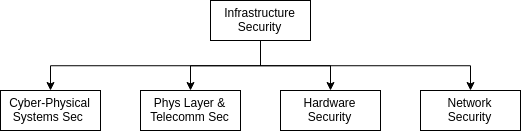
\includegraphics[width=.75\linewidth]{resource/img/ch_background/cybok_metrics/cybok_infra.png}
\end{mdframed}
\caption{Cybok: Infrastructure Domain Metrics
\label{fig:background:cybok_infra_metrics}}
\end{figure} 


Infrastructure Metrics to evaluate hardware security can be found in Rostami’s survey\cite{Rostami_2013, Rostami_Koushanfar_Karri_2014}. The majority of these are incident counts or ratios of expected to actual values, although analytical calculations (Hamming distances) are suggested to measure the amount of divergence from a known good source in several proposed metrics. Assuming the gold standard is available against which these measurements can be taken, they will evaluate the measurement empirically and deterministically. These metrics are similar to their performance related counterparts (eg, SPEC CPU) in that the performance increase over or under a reference system can be represented as a ratio of the two values. 

Cyber-Physical Systems (CPS) includes SCADA and other control systems, vehicle networks, and IoT systems that fall outside the scope of this thesis but certainly have applicable security metrics associated with attack surface and information leakage. Similarly, most aspects of the other infrastructure components listed above are captured in the system and threat model and included in the Attack \& Defense security metrics. Types of security metrics applicable here but not listed in the surveys above might include supply chain vulnerabilities, weakness to eavesdropping or side channel attacks. 



\subsubsection{Software \& Platform Security Metrics}

\begin{figure}[ht]

\begin{mdframed}
\centering
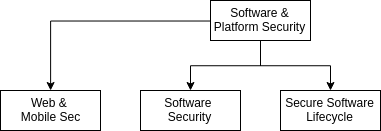
\includegraphics[width=.55\linewidth]{resource/img/ch_background/cybok_metrics/cybok_sw_platforms.png}
\end{mdframed}
\caption{Cybok: Software \& Platforms Domain Metrics
\label{fig:background:cybok_sw_metrics}}
\end{figure} 

Software security metrics were the focus of Morrison’s survey and apply here broadly. Typical applications of these type metrics derive from static analysis and test coverage. Of specific interest in the thesis is the remediation velocity, which measures the time between discovering a flaw in software and the time a fix has been merged into the code base.


\begin{figure}[ht]
\centering
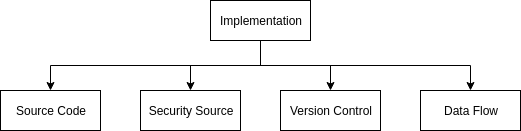
\includegraphics[width=.85\linewidth]{resource/img/ch_background/cybok_metrics/morrison_implementation.png}
\centering
\caption{Morrison’s Implementation Security metrics fall under SW\&P.
\label{fig:background:morrison_implementation_ad}}
\end{figure} 

% \subsubsection{Systems Security Metrics}

\subsection{Summary}

In the surveys summarized above there were over 500 distinct security metrics identified. The surveys each provided their own classification systems which were appropriate for the analysis they conducted, but none of these taxonomies generalize well to classify all types of security metrics. In this section we have described properties common to all metrics, identified overlaps in the various taxonomies, identified points of confusion between existing metric hierarchies, and described a suitable and intuitive system for classifying any current or future security metric. By using the Cybok as the underlying classification system we are also able to determine the distribution of metrics in each topic and identify areas of limited coverage which would benefit from future research.








% \subsection{Graph Based Metrics}\label{sec:background:graph_based_metrics}

% 



\begin{table}[ht]\centering
\caption{Metrics Summary\label{tab:metric_summary}}
% \addcontentsline{lot}{table}{Metrics Summary}
\resizebox{.8\textwidth}{!}{%
\begin{tabular}{@{}lp{.35\linewidth}l@{}}
\toprule
Metric Class & Description & Common Measurements \\ \midrule
Structural & Metrics based on the structure of the attack graph; used to identify attributes like shortest path, mean path length, or total number of paths. & SP, NP, MPL \\
Time-Based & Metrics that quantify time expectations for attributes like compromise, recovery, or incident response. & MTTF, MTTB, MTTR \\
Probability-Based & Metrics that associate probabilities attack paths to quantify the security of the network. & NR, PP, EPL \\
Temporal & Metrics that examine  vulnerability age on the system. & TAG \\ \bottomrule
\end{tabular}%
}
\end{table}

% 


\input{content/chapters/ch_background/sec_metrics/metrics_intro.tex}

\subsection{Existing Security Metrics Taxonomies}\label{sec:background:existing_metrics_taxonomies}

\input{content/chapters/ch_background/sec_metrics/existing_taxonomies}

\subsection{Security Metrics Taxonomy}\label{sec:background:metrics_by_cybok}

\input{content/chapters/ch_background/sec_metrics/sec_metrics_taxonomy.tex}

% \subsection{Graph Based Metrics}\label{sec:background:graph_based_metrics}

% \input{content/chapters/ch_background/sec_metrics/sec_metrics.tex}

% % \subsection{Metric Validation}\label{sec:background:metric_validation}

% % \input{content/chapters/ch_background/metric_validation.tex}

% % \section{Related Work}\label{sec:background:related}

% % \subsection{Structural Metrics} \label{subsec:struct_metrics}
% \input{content/chapters/ch_background/sec_metrics/structural_metrics.tex}

% % \subsection{Probabilistic Metrics} \label{subsec:prob_metrics}
% \input{content/chapters/ch_background/sec_metrics/prob_metrics.tex}

% \begin{table}[H]
% \begin{tabular}{p{3.2cm}p{8cm}p{3cm}p{3cm}}
% %{@{}llll@{}}
% \toprule
% Metric Class & Description & Common Measurements   \\ \midrule
% Structural & Metrics based on the structure of the attack graph; used to identify attributes like shortest path, mean path length, or total number of paths. & SP, NP, MPL   \\
% Time-Based  & Metrics that quantify time expectations for attributes like compromise, recovery, or incident response. & MTTF, MTTB, MTTR   \\
% Probability-Based  & Metrics that associate probabilities attack paths to quantify the security of the network. & NR, PP, EPL   \\
% Temporal & Metrics that examine  vulnerability age on the system. & TAG   \\ \bottomrule
% \end{tabular}
% \caption{Metrics Summary}
% \label{tab:metric_summary}
% \end{table}

% % \subsection{Metric Validation}\label{sec:background:metric_validation}

% % 
In \cite{Verendel_2009} Verendel finds 4 distinct validation methods used across the 90 security metrics papers surveyed: hypothetical, empirical, simulation, and theoretical. The author adds the caveat that no attempt was made to verify the quality of results, only to describe the methods used in each paper to substantiate the findings. In this thesis we demonstrate a framework for validating security metrics through empirical means. Specifically, 
\cite{Sonmez_2019}

% % \section{Related Work}\label{sec:background:related}

% % \subsection{Structural Metrics} \label{subsec:struct_metrics}
% 
Structural metrics draw conclusions about the security properties of the attack graph through basic graph analysis techniques\cite{Dacier_Deswarte_Kaaniche}\cite{Ortalo_1999}.  

\textbf{Shortest Path (SP):  }

Given an attack graph, the Shortest Path metric identifies the minimum number of nodes (vulnerabilities) an attacker would need to exploit to reach the target. Techniques for finding the shortest path in a graph are well-documented in Computer Science \cite{Dijkstra_1959}.  For the collection of paths, \(p_i\), in an attack graph \(AG\) we define the shortest path as: 

\[SP(AG) = min(len(p1), len(p2), \ldots, len(pi), \ldots, len(pn)) \]

% The shortest path metric could be used by an attacker to identify the most direct route to a target. Another consideration is that an attacker may want to determine shortest paths as part of a minimal cut set algorithm for efficiently intercepting or degrading the target’s communications. 

\textbf{Number of Paths (NP):}  

NP is a count of the unique paths that exist on an attack graph between the attacker and the target. It is a reasonable measure of the risk exposure of the network and provides a sense of how many options an attacker would have available during a targeted attack.  
\[NP = |p_1, p_2, \ldots, p_i, \ldots, p_n| \] 

\textbf{Mean Path Length (MPL): }

MPL calculates the arithmetic mean of the path lengths on the network as a way to size the average effort required to compromise a target.  

\[MPL = \frac{\sum_{i}len(p_i)}{NP(AG)}\]
 

 

While we can obtain some insight into the security properties of different attack graphs through direct comparison, there is not enough granularity in these structural metrics to determine the characteristic strengths or weaknesses of the underlying security posture. For example, we notice that there is a large discrepancy in the NPL measures among the three graphs; however, we can’t determine conclusively that this makes one model more susceptible to attack without knowing more about how each model’s vulnerability and exploitability relate. Effort has been made [12] to introduce statistical methods into structural metrics as a means for more reliable comparison. 


% % \subsection{Probabilistic Metrics} \label{subsec:prob_metrics}
% 
Attack graphs have long been modeled as probabilistic processes\cite{ Dacier_Deswarte_Kaaniche, Ortalo_1999, Phillips_Swiler_1998, Weiss_1991}. We consider the movement of an attacker through the nodes of the attack graph as a stochastic process and interpret the state of the system as the current position of the attacker in our network. An attacker can advance to another state in the process through successful compromise of the vulnerability represented by that state only if there exists an edge in the attack graph between the attacker’s current state and the advance state.  The collection of all states in the process is the system’s state space and corresponds to the set of nodes in our attack graph. Advancing to another state is probabilistic and the success of the advance is based on the weighted score associated with that node. For example, from Figure \ref{fig:tg_001}, if the attacker is at Node 3, the probability that the target will be compromised is only based on the difficulty of exploiting the vulnerability on Node 1 (Trojan installation), and not on the path the attacker took to arrive at Node 3.

Because we only need to rely on the current state of the system and not how the system arrived in that state to determine the next state, we are able to model the attack graph as a Markov Chain without loss of generality. A Markov Chain is a stochastic process that is \textit{stateless}, that is, prediction of the next system state can be made based only on the current state. This is known as the Markov Property.  

More formally, for a stochastic process \(X = {X_t, t \geq 0}\), if the attack graph has \(n\) nodes, then the set of possible states, \(S\), for \(X\) is \(S = {s_1, s_2, \ldots, s_a, \ldots, s_n}\). The probability \(P_i,j\) that an attacker in state \(X_t\) will advance to state \(X_{t+1}\) can be given as \(P(X_{t+1} = j | X_t = i)\) with the Markov Property being satisfied as: 
\[P(X_{t+1} = j | X_1 = x_1 , X_2 = x_2 , \ldots, X_t = i)  = P(X_{t+1} = j | X_t = i) \]
The value \( P_{i,j}\) is known as the transition probability between two states\( s_i\) and \(s_j\). We can model the n states of the process \(X\) as an \(nxn\) matrix whose\( (i, j) \)entry is the transition probability\( P_{i,j}\).

The transition matrix
\[
P = \begin{bmatrix} 
    P_{11} & \dots & P_{1n}  \\
    \vdots & \ddots & \\
    P_{n1} &        & P_{nn} 
    \end{bmatrix}
\]
must also satisfy the conditions:  

\[0 \leq P_{i,j} \leq 1\quad for\quad i,j \in S\]

\[\sum_{j=1}^{n} P_{i,j} = 1\]

That is, if a state has three outbound edges (possible choices to exploit next), the probability that any edge is followed is \(1\) since we must proceed to the attack goal after each time step, and the probability a specific edge is followed is determined by how exploitable that vulnerability is (the transition probability). This stochastic model enables us to study the system’s quantitative and qualitative properties through well-established analytic and simulation methods. Assuming the system state is given as the attacker’s current location on the attack graph (the vulnerability most recently exploited), we can model the system’s subsequent states through iteration of the stochastic process over discrete time intervals.  

 

Attack graphs in general have the special property that the attack goal can be reached from any node in the network, allowing us to model them as an Absorbing Markov Chain using the transition matrix described above. An Absorbing Markov Chain is a Markov Chain that includes at least one absorbing state, in our case the attack goal. The absorbing state can be reached from all other states, and once the absorbing state is reached (the attacker has compromised the target), no further transitions are considered.  

\begin{figure}[ht]
\centering
\includegraphics[width=.8\textwidth]{resource/img/ch_background/sdn_analytics/eg_trans_diagram.png}
%%\includegraphics[width=100mm]{content/figs/eg_trans_diagram.png}
\caption{Example Transition Diagram}
\label{fig:ag_2}
\end{figure} 

In Figure \ref{fig:ag_2} we see a  notional transition diagram. The possible states in the chain are connected by edges labeled with the probability of advancing to an adjacent state (successfully exploiting the next vulnerability.) The self-referencing edges represent the probability of an unsuccessful exploit and occur at entries \(Pi,i\) along the diagonal of the transition matrix. Note that once the system enters the ‘Target’ state no other state is reachable which we define as the absorbing state.  

 

To create a transition matrix that conforms to the definition of an absorbing Markov chain, each outbound edge is assigned a transition probability calculated by normalizing the CVSS exploitability scores associated with all adjacent (next-step) states. That is, if we are at state \(S_i \)and the set of possible next states are given as \(S_{i+1} = {s1, s2, \ldots, sn}\) then we calculate the transition probability
\[ Pij =\frac{CVSS(s_j)}{\sum_{k=1}^{n}CVSS(s_k)}; k \in S_{i+1}\]
This normalizes the transition probabilities for all outbound states of a given node and guarantees the two conditions for a Markov transition matrix defined above will be satisfied.  

 

The transition matrix \( P\) for the absorbing Markov chain defined above can be put into the canonical form \( P=\)
\(\begin{bmatrix}
Q & R \\
0 & I
\end{bmatrix}\)
  where \(Q\) is the matrix of transition probabilities for moving from a non-absorbing (transient) state to another transient state, and \(R\) is the matrix of transition probabilities for moving from a transient state to an absorbing state. In other words, we can order the rows and columns such that all transient states precede the absorbing states.  

 

From the canonical form, \(P_k\) approaches some limiting matrix \(|P|\) as \(k\) increases, where\( |P|=\)
\(\begin{bmatrix}
0 & FR \\
0 & I
\end{bmatrix}\)
  and \(F = (I-Q)-1\). This matrix \(F\) is known as the fundamental matrix for \(P\), and it allows us to derive many interesting properties from our system. For example, the\( (i, j)\) entries of \(|P|\) provide the long-term (limiting) probabilities of advancing from state \(i\) to state \(j\). Likewise, the sum of the row  entries in \(F\) determine the average number of steps it will take to reach an absorbing state from each transient state. 

Note that for the transition matrix \(P\) defined above, the entry \(P_{i, j}\) is the probability the system given initial state \(s_i\) will move to state \(s_j\) on the next step. It follows from the total probability theorem that the probability the system will be in state \(s_j\) after exactly two time steps is the \((i, j)\) entry of:  
\[
P^2=
\begin{bmatrix}
Q & R \\
0 & 1
\end{bmatrix}
\begin{bmatrix}
Q & R \\
0 & 1
\end{bmatrix}=
\begin{bmatrix}
Q^2 & QR + R \\
0 & 1
\end{bmatrix}
\]
After 3 time steps:
\[
P^3=
\begin{bmatrix}
Q^2 & QR + R \\
0 & 1
\end{bmatrix}
\begin{bmatrix}
Q & R \\
0 & 1
\end{bmatrix}=
\begin{bmatrix}
Q^3 & Q^2R +QR + R \\
0 & 1
\end{bmatrix}
\]

 
 …, and after t time steps: 
 \[
P^t=
\begin{bmatrix}
Q^t & (I + Q +Q^2 ... +Q^{t-1}) R \\
0 & 1
\end{bmatrix}
\]
 We have defined \(Q\) as the matrix of transient probabilities with values less than \(1\), so it holds that \(Q^t \to 0\) as \(t \to \infty\)
(eventually we will reach the attack target). Now consider the matrix  \(F\) such that \( F= I + Q + Q^2 +...\)

The values of \(Q^t(i,j)\)  then are the probabilities of the system starting in state \(s_i\) and ending in state \(s_j\) exactly \(t\) steps later. In this case we can interpret the probability \(Q^t(i,j)\)
  as the fraction of time period \(t\) spent in state \(s_j\), so the total number of periods the process occupies state \(s_j\) before becoming absorbed is:  \(F(i, j) = Q^0(i,j)+Q^1(i,j)+Q^2(i,j)...\) and the reduced form is known as the \textbf{fundamental matrix:}
\[ F = (I-Q)-1\] 


% we have scripted the process of parsing the MulVal output, reducing and coalescing the nodes into a format compatible with the Cyber Security Analytics Framework, performing the lookup of CVSS scores for known vulnerabilities, and calculating the transition probabilities. 

% *The transition matrix provides a key input for stochastic modeling, which will be used to produce the final metrics through simulation or analytical means. 

% *Finally, the attack graph encoded with the desired transition probabilities is used as input for the metric derivation model, in this case using Markov chains. The model is run under simulation or solved analytically to produce the desired metric output suitable for comparison.  

%  The result is the fundamental matrix used as input to stochastic models to calculate the various metrics.  


% Section \ref{sec_contributions} details the design and implementation with a supporting case study in section \ref{sec_approach}. 

\textbf{Node Ranking (NR):  }

We have shown that the elements of the fundamental matrix \(F\) take on values that represent the relative duration of time spent at each transient node in the Markov process. In the context of our security analysis, these values equate to the amount of hold time we expect an attacker to incur while trying to advance to the target. Lower node rankings indicate nodes along the attack path that are relatively easy for an attacker to clear. If a difficult to exploit vulnerability exists and its associated NR is relatively low this might be an indication that a security control point is being bypassed. Using the attack graph and associated NR analysis it is a fairly straight forward process to identify the area of interest and trace back to the origin of the bypass. Liu\cite{Liu_Singhal_Wijesekera} examines this process of forensic reconstruction of attacks using attack graphs in detail.

\textbf{Probabilistic Path (PP):} 

The PP metric is another interesting property derived from our Markov transition matrix. Taking the product of the fundamental matrix F and the matrix of absorbing probabilities \(R\) results in a matrix, \(B = FR\), whose \(B(i,j) \) entries yield the probability of being absorbed by state \(s_j\) given we started at initial state \(s_i\).  

\textbf{Expected Path Length (EPL):  }

We define EPL as the expected number of time steps required for an attacker to advance from the initial state to the attack goal, and its calculation follows as a direct consequence of deriving the NR metric. That is, if the NR metric expresses the total expected time that a process starting in initial state $s_i$ will occur in transient state \(s_j\) before ultimately being absorbed, then the NR sum over all transient states for \(s_i\) will predict the total time spent in the process before absorption. To take the sum of the values in the rows of the fundamental matrix we multiply by a column of 1’s, $t = N1$, and the entry \(t_i\) contains the EPL value for initial state \(s_i\). 
 

\textbf{Mean Time To Failure (MTTF)} 
Time based metrics are a subset of probabilistic measures used to estimate how long it will take for some target objective to be met.
MTTF is the measure of the mean time for an attacker to reach a target. This measure directly maps to Expected Path Length as we have defined it. 


% \begin{table}[H]
% \begin{tabular}{p{3.2cm}p{8cm}p{3cm}p{3cm}}
% %{@{}llll@{}}
% \toprule
% Metric Class & Description & Common Measurements   \\ \midrule
% Structural & Metrics based on the structure of the attack graph; used to identify attributes like shortest path, mean path length, or total number of paths. & SP, NP, MPL   \\
% Time-Based  & Metrics that quantify time expectations for attributes like compromise, recovery, or incident response. & MTTF, MTTB, MTTR   \\
% Probability-Based  & Metrics that associate probabilities attack paths to quantify the security of the network. & NR, PP, EPL   \\
% Temporal & Metrics that examine  vulnerability age on the system. & TAG   \\ \bottomrule
% \end{tabular}
% \caption{Metrics Summary}
% \label{tab:metric_summary}
% \end{table}